%This chapter introduces and explains the fundamentals to understand the rest of the this disseration. Firstly, Mapping and Localization technologies are explored and then an explanation on to use them in \acs*{SLAM} is provided. Finaly, several \acs*{SLAM} implementations and related works are discussed and compared.

From the beginning of civilization, mapping the surroundings has been a key concept for navigating the environment. In essence, the problem our ancestors faced is currently being tackle in robotics: How do we map the environment and know our location within it? This is a massive problem to tackle on and of extreme importance to achieve full robot autonomy. In a simple approach, a depth sensor in a static platform is enought to map the surroundings, this is the base platform of the taxometry chart presented in Figure \ref*{fig: taxonomy graph}. At this level localization is not needed, but the amount of uses in real world are skew. The next level presents a localization component, this allows the usage of mobile robot's to map the environment. If the localization information is correct, precise and without any uncertainty associated this would be enough to generate an accurate map. However, this scenario is not reallistic. The more complex level presents a two way communication between the mapping and localization, this is often refered as \acl*{SLAM}. \acs*{SLAM} is the challenge of mapping the local environment of a moving entity (e.g. robot) and updating the map and localization simultaneously and continuously as the entity moves through space.

\begin{figure}[H]
    \centering
    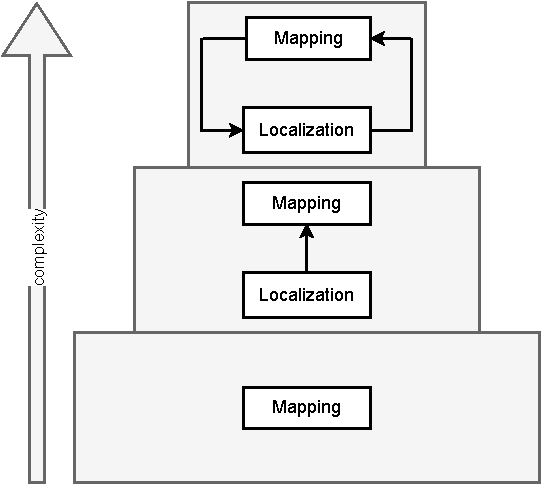
\includegraphics[width=0.4\linewidth]{images/background/mapping taxo.pdf}
    \caption{Mapping taxonomy graph}
    \label{fig: taxonomy graph}
\end{figure}


\section{Mapping}

Maps in robotics are usually represented either metrically or topologically. The information on topological maps is presented in the form of a graph that contains all of the important landmarks.In the metric representation, everything above the resolution of the map appears on the map. A metric map can be represented with raw sensor measurements or occupancy grids, the latter being more common. In occupancy grids, each cell holds the probability that the space in that cell is currently occupied. As the cell value increases, the likelihood of that space being occupied also increases. The resolution of the map will be determined by the size of the grid, therefore to generate a precise map, one must have large dedicated memory space, which presents an inconvenience and this is the most significant drawback of metric maps. Octomap is a popular 3D mapping framework to generate occupancy grids based on depth information \cite{hornung_octomap_2013}. Octomap uses octrees\footnote{An octree is a tree data struture in which each internal node is subdivided in eight children until the structure resolution is met.} to help reduce the memory space of rendering a map since large spaces with equal values can be represent with a single parent node.

\section{Localization}
Localization can take two forms: global or relative. Global localization gives the position in a global reference. Information provided by global localization can be viewed independently of other positions.
Relative localization, as the name suggests, the current pose (position and orientation) is related to other pose. A pose's current state is usually determined by its last state. To estimate change in poses over time it is common to use data from motion sensors, such as wheel encoders and \acs*{IMU}s. The procedure of estimating a change in pose over time by using sensory information is called odometry. 
Many times sensor information is too noisy to be directly use as an input, which is a problem. A common way to solve this problem is to use a Kalman filter.

\subsubsection{Kalman Filter}
The Kalman filter is a \textbf{linear} iterative process based on Bayes Theorem, that uses consecutive data input to quickly converge to the true value. Each iteration involves computing three values: the Kalman gain, the current estimate, and its uncertainty. The estimate of the current iteration is computed with the new data input and the previous estimation, where the weight of each component is decided by the kalman gain. Once the current estimate has been calculated, the new uncertainty of the estimate is computed. One can think of the Kalman Gain as a variable that represents the confidence one has in the observations and predictions made. Figure \ref*{fig: flowchart kalman} provides a simple graphical overview of this process. A more complete explanation of the statistics envolved in the Kalman filter is provided in Annex. 

\begin{figure}[H]
    \centering
    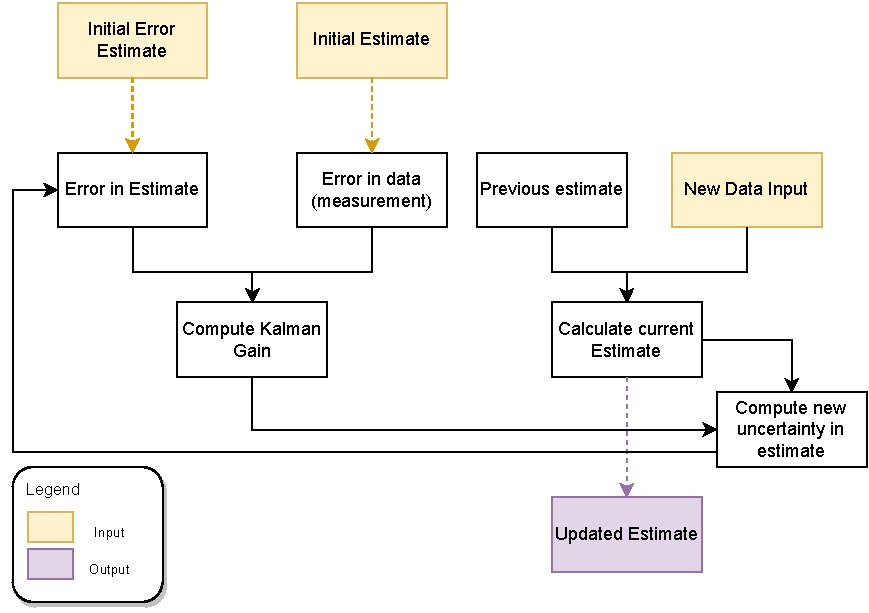
\includegraphics[width=0.5\linewidth]{images/background/Kalman-diagram.pdf}
    \caption{Simple flowchart of the Kalman Filter.}
    \label{fig: flowchart kalman}
\end{figure}

In real world it is uncommon to have a global linear system and due to it's linearity, the Kalman Filter won't work well in nonlinear scenarious. A simple way to solve this is to make the global nonlinear function, locally linear, using a first order Taylor Expansion to do the aproximation. This is the approach taken by the \acl{EKF} (\acs*{EKF}) method. A more accurate way to solve the problem is to use a \acl*{UKF} (\acs*{UKF}). Instead of linearizing the original function, the \acs*{UKF} uses an Unscented Transformation\footnote{The Unscened transform picks a few points from the distribution of the input variable, then it passes them through the nonlinear function and computes the mean and standard deviation of the output. A complete explanation is given in Annex}. A problem still remains, the noise is assumed to follow a gaussian distribution in every Kalman filter approach, which is not necessarely true. A alternative method, that works with non-Gaussian \acl*{PDF} (\acs*{PDF}) is the Particle Filters method.

\subsubsection{Particle Filters}

The Particle Filter is an iterative linear method is based on the Monte Carlo approach. Essentially, this method describes any complex \acs*{PDF} as a group sample points. The sample points can be see as guesses of the true value. The higher density of points in a location, the higher the probability. The weigth is then computed based on the observations made and finally a resample is made to discard low probability points.

\section{\acs*{SLAM} techniques}

Now that both localization and mapping were reviewed, the techniques to merge them together in \acs*{SLAM} can be presented. As mentioned before, sensors used to capture information of the real world have uncertainties associated with each measurement. Even when algorithms are implemented to diminish these errors, they never vanish completely. When performing \acs*{SLAM}, a moving robot's perception and performance can be severely affected by these inaccuracies as they accumulate and become increasingly large. In the case of a pose error, in each iteration odometry information is combined with the previous pose, both of which are subject to uncertainty. Over time, the cumulative error of the robot will increase significantly. A way to reduce is to establish a two way communication between the localization and mapping component. Classical odometry is computed from motion sensors such as \acs*{IMU} or wheel encoders, but it is also possible to use cameras as an input to acquire odometry, this is called visual odometry. Feature matching algorithms (identifying and relating the same features of an object from different perpectives) like ORB \cite{rublee_orb_2011} are at the core of many Visual Odometry algorithms, recently Liu et al. \cite{liu_visual_2021} developed a Visual Odometry algorithm based on a Deep Learning technique. Another way to acquire odometry is by using \acs*{LiDAR}s and a scan matching algorithm like the \acl*{ICP} method (\acs*{ICP}). Scan matching takes two pointclouds or 2D \acs*{LiDAR} scans and finds the transformation that produces the least amount of error between points. Simply put, it tries to transform in a way to overlap the information of both scans, the transform is then applied to estimate the robots location, as is shown in Figure \ref*{fig: scan mathing algorithm}. Both scan matching and feature matching can be used to find a transform to update the localization of the robot, Figure \ref*{fig: scan mathing algorithm} shows how scan matching can be used to update the robot location with information of the map.

\begin{figure}[H]
    \centering
    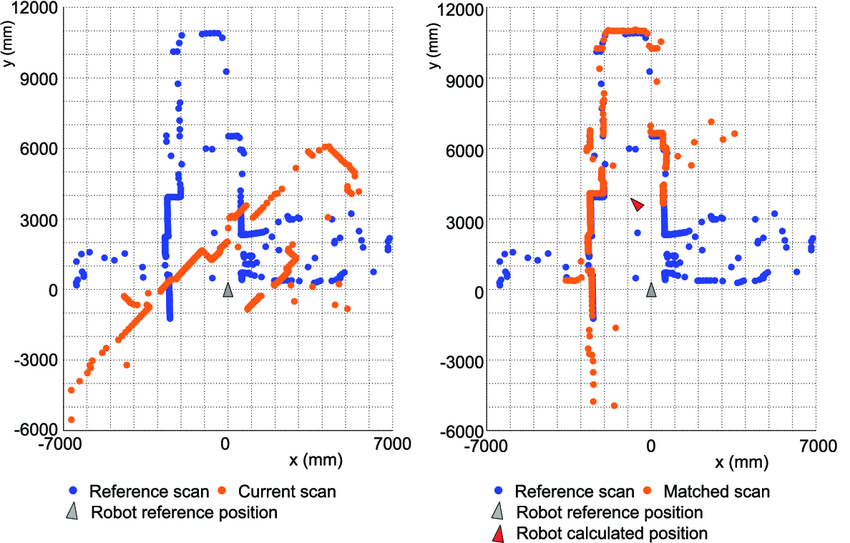
\includegraphics[width=0.7\linewidth]{images/background/Scan-matching-problem-definition-a-Scans-before-alignment-b-Scans-after-alignment.png}
    \caption{Scan matching to calculate a robot position. \cite{konecny_scan_2019}}
    \label{fig: scan mathing algorithm}
\end{figure}

\subsubsection{Loop Closure}

The capacity of the system to recall previously visited landmarks is regarded as loop closure. Loop closure identifies a previously mapped location and through feature or scan matching algorithms updates the robot location. This will significantly reduces the error in localization, since the cumulative error of in the pose is discarded. One can think of loop closure as a reset of the pose uncertainty whenever the robot passes through a previously known location. However, an inaccurate detection of a loop closure will introduce a large error in both the mapping and robot's localization, so one must be sure the landmarks are properly identified.

\subsection{Filter based \acs*{SLAM}}

Filtering based \acs*{SLAM} employs the filtering techniques described previously, namely Kalman Filters and Particle Filters. The \acs*{EKF} \acs*{SLAM} is one way to solve the \acs*{SLAM} problem using the previously explained \acl*{EKF}. As it uses the \acs*{EKF}, each map and pose must linearly dependent of the previous iteration and this is major shortcome. If the robot moves at a constant speed we can assume the change in pose to be linear. This will not be the case as the robot often accelerates, but if the acceleration is not abrupt the nonlinear system will be succefully approximated to linear by means of a first order Taylor expansion. The biggest drawback is the implied assumption of a static map. Moving entities in the environment will obviously not produce a close to linear dependency in succeful iterations, therefor the first order Taylor expansion will not yield good results. 


The FastSLAM algorithm \cite{thrun_fastslam_nodate} uses particle filters to estimate the change in pose of the robot. By using Particle Filters, FastSLAM can handle nonlinear robot motion but it is more computive intensive. Another advantage of using a Particle Filter to estimate the motion is the multiple system states that are kept in memory through the resampling process, that only discards the low probability states. There are also implementations which replace the \acs*{EKF} by the \acs*{UKF} method to update the landmarks \cite{wang_upf-ukf_2007}.


\subsection{Graph-based \acs*{SLAM}}

The graph-based \acs*{SLAM} technique, initially proposed by Lu and Milios et al. \cite{lu_globally_1997}, uses a graph-based approach, in which nodes represent poses or landmarks, while edges represent constraints between nodes, typically obtained from odometry or loop closure techniques, as illustrated in Fig. \ref*{fig: graph SLAM}. Unlike the filtering approach, the graph-based technique maintains knowledge on all gathered data and uncertainties are encoded in the graph. This approach divides \acs*{SLAM} into two main problems: graph construction (building the graph from sensory information, commonly known as front-end) and graph optimization (analysing and estimating the most likely global configuration of poses given the constraints, also known as back-end).

\begin{figure}[H]
    \centering
    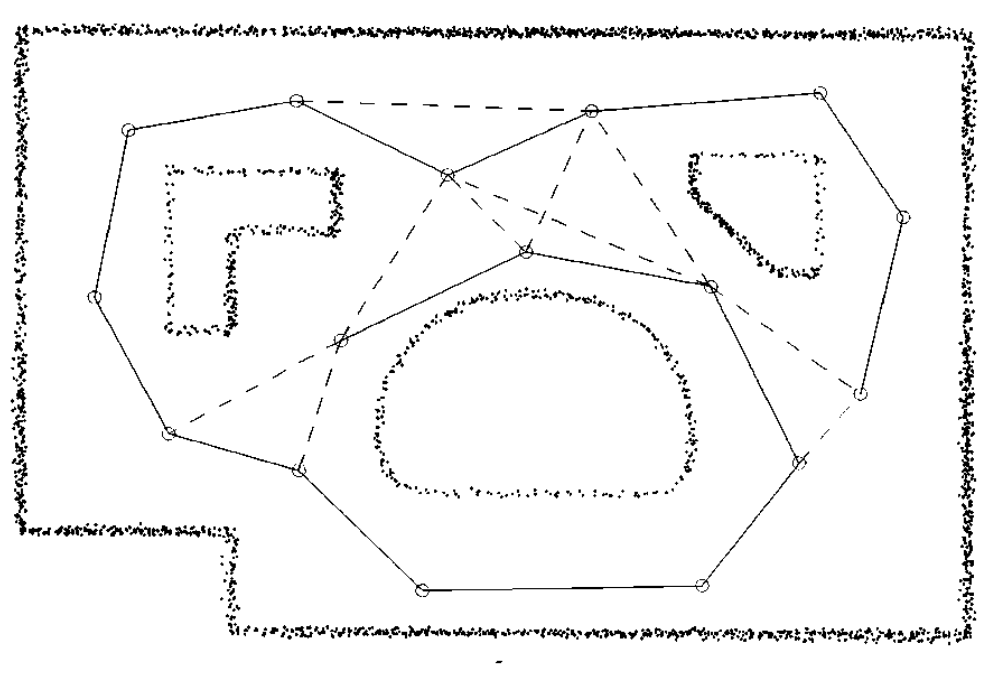
\includegraphics[width=0.7\linewidth]{images/background/graph_SLAM.png}
    \caption{A pose-graph representation of \acs*{SLAM}. The circles represent the robot's poses, the solid lines are constrains derived from odometry and the dotted lines are from scan matching constrains \cite{lu_globally_1997}.}
    \label{fig: graph SLAM}
\end{figure}

Every new pose introduces a new node into the graph with multiple constraints associated, the constrains can be divided into \textit{weak links} provided by odometry data and \textit{strong links} obtained from scan or feature matching algorithms. These links can be viewed as elastic springs with different elastic constants \cite{lu_globally_1997}, the global graph optimizer will then find the lowest energy solution to the system. To put it simply, the frontend is responsible for generation of accurate submaps, while the backend ensures they are consistently correlated.

\section{\acs{ROS}}

An effective robotics project cannot be achieved by just having sensors and physical components; rather, one must have a clever communication system between sensors and processes. This task can be carried out by the \acl*{ROS} (\acs*{ROS}). 

Although the name \acl*{ROS} suggests that \acs*{ROS} is an operating system, this is not the case.  In a way, \acs*{ROS} is both middleware and a framework. The system provides a communication channel where messages can be easily subscribed, published and distributed, allowing quick integration between systems and components. Moreover, it provides features such as debugging, visualization, testing, logging, and configuration right out of the box. Additionally, ROS includes a number of useful packages for essential areas relevant to robotics such as movement, perception, and manipulation. The ROS community is also constantly evolving with the most recent developments in robotics, so libraries are always being added to ROS. Many of these libraries are open-source implementations of previously described \acs*{SLAM} techniques, these libraries will now be reviewed and compared.


\section{\acs*{SLAM} implementations in \acs*{ROS}}

There are a multitude of open source implementations of \acs*{SLAM}. Since one of the \textbf{Must} requirements is a well integrated system with the \acs*{ROS} platform, only \acs*{ROS} implementations will be reviewed. 

One of the most popular implementations of \acs*{SLAM} is Real Time Appearance Based Mapping (RTAB-Map) \cite{labbe_rtab-map_2019}. RTAB-Map\footnote{The \acs*{ROS} implementation can be found at \url{https://github.com/introlab/rtabmap}} is a graph-based \acs*{SLAM} that uses loop closure detector and offers several options for the backend, namely GTSAM (default) \cite{gtsam}, g2o \cite{kummerle_g2o_2011} and TORO \cite{grisetti_nonlinear_2009}. It supports several sensors, namely \acs*{LiDAR}, RGB-D and stereo cameras. It can gather odometry from \acs*{IMU} and wheel encoders but it also supports Visual and \acs*{LiDAR} odometry as optional sources. In order to ensure offline\footnote{In literature, real-time \acs*{SLAM} is referred to as offline \acs*{SLAM} and heavy implementations that are not meant to run in real-time are referred as online \acs*{SLAM}} \acs*{SLAM}, RTAB-Map has a memory manager that keeps control of the amount of locations and landmarks used in the loop closure. Additionally, when executing the loop closure, RTAB-Map will reuse the features that were previously matched in Visual or \acs*{LiDAR} Odometry, this also contributes for performance. RTAB-Map can generate both 2D and 3D Occupancy grids with Octomap.

Several \acs*{LiDAR} based method derive from \acl*{LOAM}, commonly known as \acs*{LOAM}. Implementations based on \acs*{LOAM} usually both odometry and mapping from \acs*{LiDAR}. Although it can create high accuracy maps, the maps are static and it usually performs poorly in places with few landmarks, like long corridors. The LeGO-LOAM\footnote{The \acs*{ROS} package can be at \url{https://github.com/RobustFieldAutonomyLab/LeGO-LOAM}} add two aditional modules to the \acs*{LOAM} technique: pointcloud segmentation and loop closure. These extra components allow a improvement in computing performance and drift reduction over long distances but doesn't improve the results when used in a featureless enviroment. LeGO-LOAM uses the naive \acs*{ICP} algorithm to perform loop closure, but a more robust approach, based in a point cloud descriptor is implemented in the SC-LeGO-LOAM\footnote{The \acs*{ROS} package can be at \url{https://github.com/irapkaist/SC-LeGO-LOAM}} \cite{kim_scan_2018}. To help improving the performance in low features environment, researchers started to implement an \acs*{IMU} to the system in a tighly coupled approach \cite{ye2019tightly}, \cite{xu_fast-lio_2021}, \cite{xu_fast-lio2_2021}. As it was very computed intensive to take all sensory data, the authors in \cite{liosam2020shan} sugested the \acl*{LIO-SAM} (\acs*{LIO-SAM}\footnote{The \acs*{ROS} package can be at \url{https://github.com/TixiaoShan/LIO-SAM}}).

Cartographer is Google's implementation to solve the \acs*{SLAM} challenge \cite{hess_real-time_2016}. It is another \acs*{LiDAR} based graph \acs*{SLAM} divided into two main components: local \acs*{SLAM} (the front end) and global \acs*{SLAM} (the backend). This approach takes input of range finding sensor, like \acs*{LiDAR}, and applies a bandpass filter to the input data. \acs*{IMU} can also be used to help figuring out the robot rotation and to provide information on gravity direction, that is used in the 3D variant.
 
\section{Related Data Acquisition Apparatus}

It is no surprise that there are already a number of portable and light sensors designed to collect sensor data about the environment around us. There are several proprietary solutions available on the market for gathering sensory information for \acs*{SLAM}, but they tend to be expensive \cite{libackpack_C50}, \cite{libackpack_DGC50}. Additionally, there are some articles and research papers that have been conducted with the goal of building a system similar to the one proposed here. These works will be the ones to be focused on since the methodology, and results are readily available.

There exist multiple ways to scan a forest, Oveland et al. \cite{oveland_comparing_2018} compared three different ground LiDAR scanning implementations, namely, Handeld LiDAR, Backpack LiDAR (composed by two \acs*{LiDAR} perpendicular to each other) and Terrestial LiDAR. The authors compared the measurements of \acs*{DBH} to conclude that while the Terrestial LiDAR Scanners (a fixed system) is the most accurate but it fails to detect ocult areas. According to the authors the handheld LiDAR scanner has troubles in detecting smaller trees. Even tho the backpack LiDAR has the highest number of false trees, the authors still aknowledge it as the most efficient method since it presents the highest amount of trees detected and low \acs*{RMSE} of $0.022m$.

Recently, Kui Xao developed a dual \acs*{LiDAR}s system, an \acs*{IMU}, and \acs*{GPS} for performing \acs*{SLAM} in multi-scene applications \cite{xiao_high-precision_2022}. To increase the vertical \acl*{FOV} (\acs*{FOV}), one of the \acs*{LiDAR}s was placed in the \textit{XY} plane while the other was positioned at -77.94° from the \textit{XY} plane. A timestamp synchronization algorithm helped the authors merging the 3D scans from both \acs*{LiDAR}s. Secondly, the \acs*{LiDAR} data is tightly coupled with the IMU data in order to reduce noise caused by the inaccuracy of \acs*{LiDAR}-based odometry. In outdoor tests, the \acs*{IMU} calibration is improved by loosely coupling \acs*{GPS} to the \acs*{IMU} during outdoor tests. While their framework outperformed the LeGO-LOAM and LIO-SAM in indoor enviroment it failed to produce any meaningfull diference in an outdoor setup. In forest environments, on the other hand, can be expected to show a slight improvement due to the high trees that can be detected by the vertical LiDAR, adding additional features.
Based on an Ouster OS0-128 \acs{LiDAR} and a RealSense D435i, both with an integrated \acs{IMU}, Alexander Proudman's system performs online \acs{SLAM} and estimates \acl{DBH} (\acs*{DBH}) using the data collected \cite{proudman_online_2021}. While their application has the benefit of having a built-in display that allows real-time visualization of data, one of its major drawbacks is the way they build their apparatus, opting for a metal stick rather than a backpack type of design. For estimating \acs*{DBH} in an experimental setup the system presents a \acs*{RMSE} of 0.07m not considering outliers and 0.14m with outliers. As the authors acknowledge, user fatigue may lead to excessive variations in stick position, resulting in unintelligible and uncontrolled movements, damaging the performance of the apparatus. This would not be an issue if a more ergonomic structure was used. The errors due to user fatigue can be a slightly mitigated by performing \acs{SLAM} in several sessions instead of one, allowing the user to rest between shorter sessions. After recording multiple sessions, \acs*{GPS} information is used to assemble the multiple sessions's map into a single map.

Yanjun Su et al. \cite{su_development_2021} developed an accurate backpack with dual \acs*{LiDAR} positioned orthogonally for forest inventory. This system consists of two Velodyne Puck VLP-16 \acs*{LiDAR}s, an \acs*{IMU}, and a display for viewing the generated point clouds in real time. The system was designed to not be \acs*{GPS} dependent. Using an open-source Python package, the researcher claims to have achieved an \acs*{RMSE} of 0.02m, a value slightly lower than Alexander's. Due to its vertical \acs*{LiDAR}, the system was also able to estimate the height of trees, obtaining a RMSE of 1.9m but with a $R^2$ of only 0.65.

Sier et. al \cite{sier_benchmark_2022} design an apparatus with the objective to compute ground truth for trajectory in GNSS denied environments. The apparatus features six different \acs*{LiDAR}, with both spinning and solid state technologies and a stereo fish eye camera. The authors compare different state of the art \acs*{LiDAR} based \acs*{SLAM} with different \acs*{LiDAR} configurations to assess the best overall combination. The author concludes that the most robust combination is the FAST-LIO \cite{xu_fast-lio_2021} implementation using the more precise OS0 and OS1 spinning \acs*{LiDAR}s. It also reached to the interested conclusion that on outdoor environment the solid state \acs*{LiDAR}s had a similiar performance againts the more expensive counterparts. This is to be expected as the number of features in outdoor environment is considerably larger.
 
Table \ref*{tab: compare apparatus} offers a comparison between the several apparatus reviewed. As one is able to see, the apparatus focused in forest aplication don't compare multiple \acs*{SLAM} implementations, being more focused in determing the \acs*{DBH} of trees. Some of the forest focused apparatus send the recorded footage to an cloud base system to perform \acs*{SLAM} like GeoSLAM Hub\footnote{GeoSLAM Hub is a \acs*{SLAM} cloud provider, producing a map based on 3D data received. The \acs*{SLAM} algorithm used is not described}. Of all the implementations discussed only one uses a RGB-D camera, a critical component to perform combustible material identification and trees species and objects identification.

\begin{table}[H]
    \centering
    \resizebox{\textwidth}{!}{%
    \begin{tabular}{|c|cccc|c|c|c|c|c|}
    \hline
    \multirow{2}{*}{\textbf{Implementation}} &
      \multicolumn{4}{c|}{\textbf{Inputs}} &
      \multirow{2}{*}{\textbf{Display}} &
      \multirow{2}{*}{\textbf{\begin{tabular}[c]{@{}c@{}}Structure\\ Type\end{tabular}}} &
      \multirow{2}{*}{\textbf{SLAM Used}} &
      \multirow{2}{*}{\textbf{Forestry Application}} &
      \multirow{2}{*}{\textbf{RMSE of DBH}} \\ \cline{2-5}
     &
      \multicolumn{1}{c|}{RGB-D} &
      \multicolumn{1}{c|}{IMU} &
      \multicolumn{1}{c|}{LiDAR} &
      GPS/GNSS &
       &
       &
       &
       &
       \\ \hline
    Oveland &
      \multicolumn{1}{c|}{$\times$} &
      \multicolumn{1}{c|}{\checkmark} &
      \multicolumn{1}{c|}{\checkmark} &
      \checkmark &
      $\times$ &
      Backpack &
      GeoSLAM Hub &
      \checkmark &
      0.022m \\ \hline
    Xiao &
      \multicolumn{1}{c|}{$\times$} &
      \multicolumn{1}{c|}{\checkmark} &
      \multicolumn{1}{c|}{\checkmark} &
      \checkmark &
      \checkmark &
      Backpack &
      \begin{tabular}[c]{@{}c@{}}LeGO-LOAM, LIO-SAM,\\ HSDLIO\end{tabular} &
      $\times$ &
      N.A \\ \hline
    Proudman &
      \multicolumn{1}{c|}{\checkmark} &
      \multicolumn{1}{c|}{\checkmark} &
      \multicolumn{1}{c|}{\checkmark} &
      \checkmark &
      \checkmark &
      Stick &
      Graph-based SLAM &
      \checkmark &
      0.07m//0.14m \\ \hline
    Su &
      \multicolumn{1}{c|}{$\times$} &
      \multicolumn{1}{c|}{\checkmark} &
      \multicolumn{1}{c|}{\checkmark} &
      $\times$ &
      \checkmark &
      Backpack &
      N.A &
      \checkmark &
      0.02m \\ \hline
    Sier &
      \multicolumn{1}{c|}{$\times$} &
      \multicolumn{1}{c|}{\checkmark} &
      \multicolumn{1}{c|}{\checkmark} &
      \checkmark &
      $\times$ &
      Wheel Cart &
      \begin{tabular}[c]{@{}c@{}}LeGo-LOAM, FAST-LIO, \\ Livox-Mapping, LIO-LIVOX\end{tabular} &
      $\times$ &
      N.A \\ \hline
    \end{tabular}%
    }
    \caption{Comparative table of the several apparatus reviewed in this section}
    \label{tab: compare apparatus}
\end{table}

\begin{figure}[H]
    \centering
    \begin{subfigure}{0.45\textwidth}
        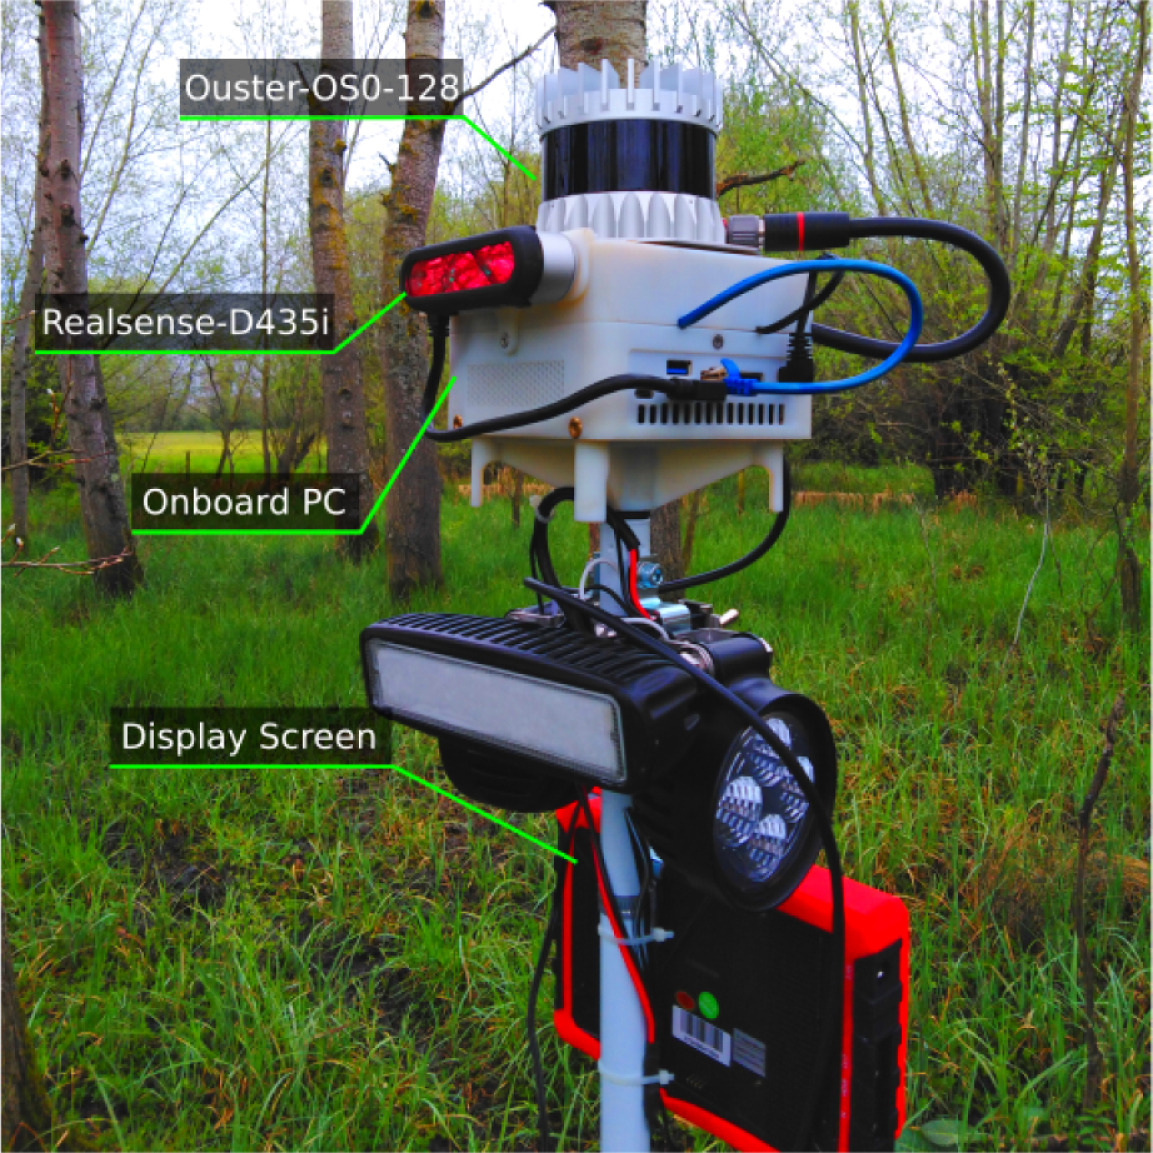
\includegraphics[width=0.8\linewidth]{images/background/alexandar_apparatus.jpg}
        \caption{Alexander's apparatus \cite{proudman_online_2021}}
        \label{fig: Alexander apparatus}
    \end{subfigure}
    \begin{subfigure}{0.45\textwidth}
        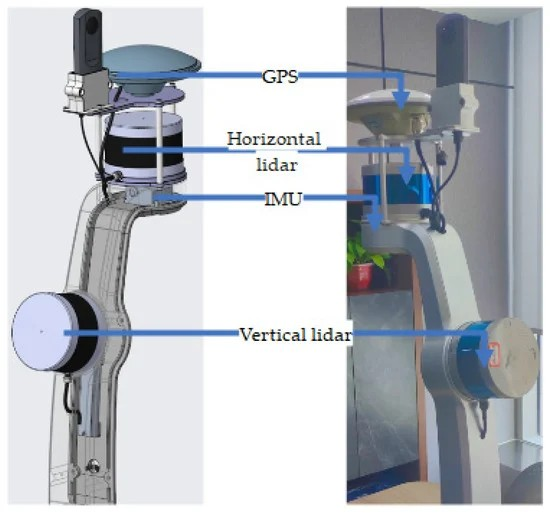
\includegraphics[width=0.875\linewidth]{images/background/xiao_apparatus.jpg}
        \caption{Xiao's apparatus \cite{xiao_high-precision_2022}}
        \label{fig: Xiao apparatus}
    \end{subfigure}
    \\[3ex]
    \begin{subfigure}{0.9\textwidth}
        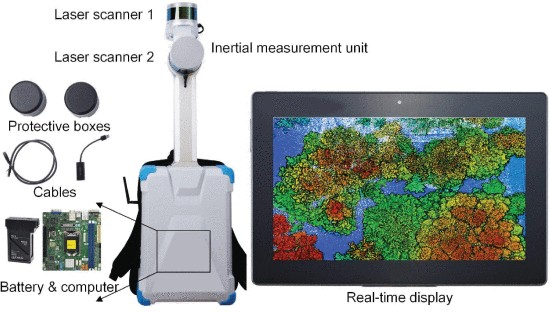
\includegraphics[width=\linewidth]{images/background/su_apparatus.jpg}
        \caption{Yanjun's apparatus \cite{su_development_2021}}
        \label{fig: yanjun apparatus}
    \end{subfigure}
    \\[3ex]
    \begin{subfigure}{0.45\textwidth}
        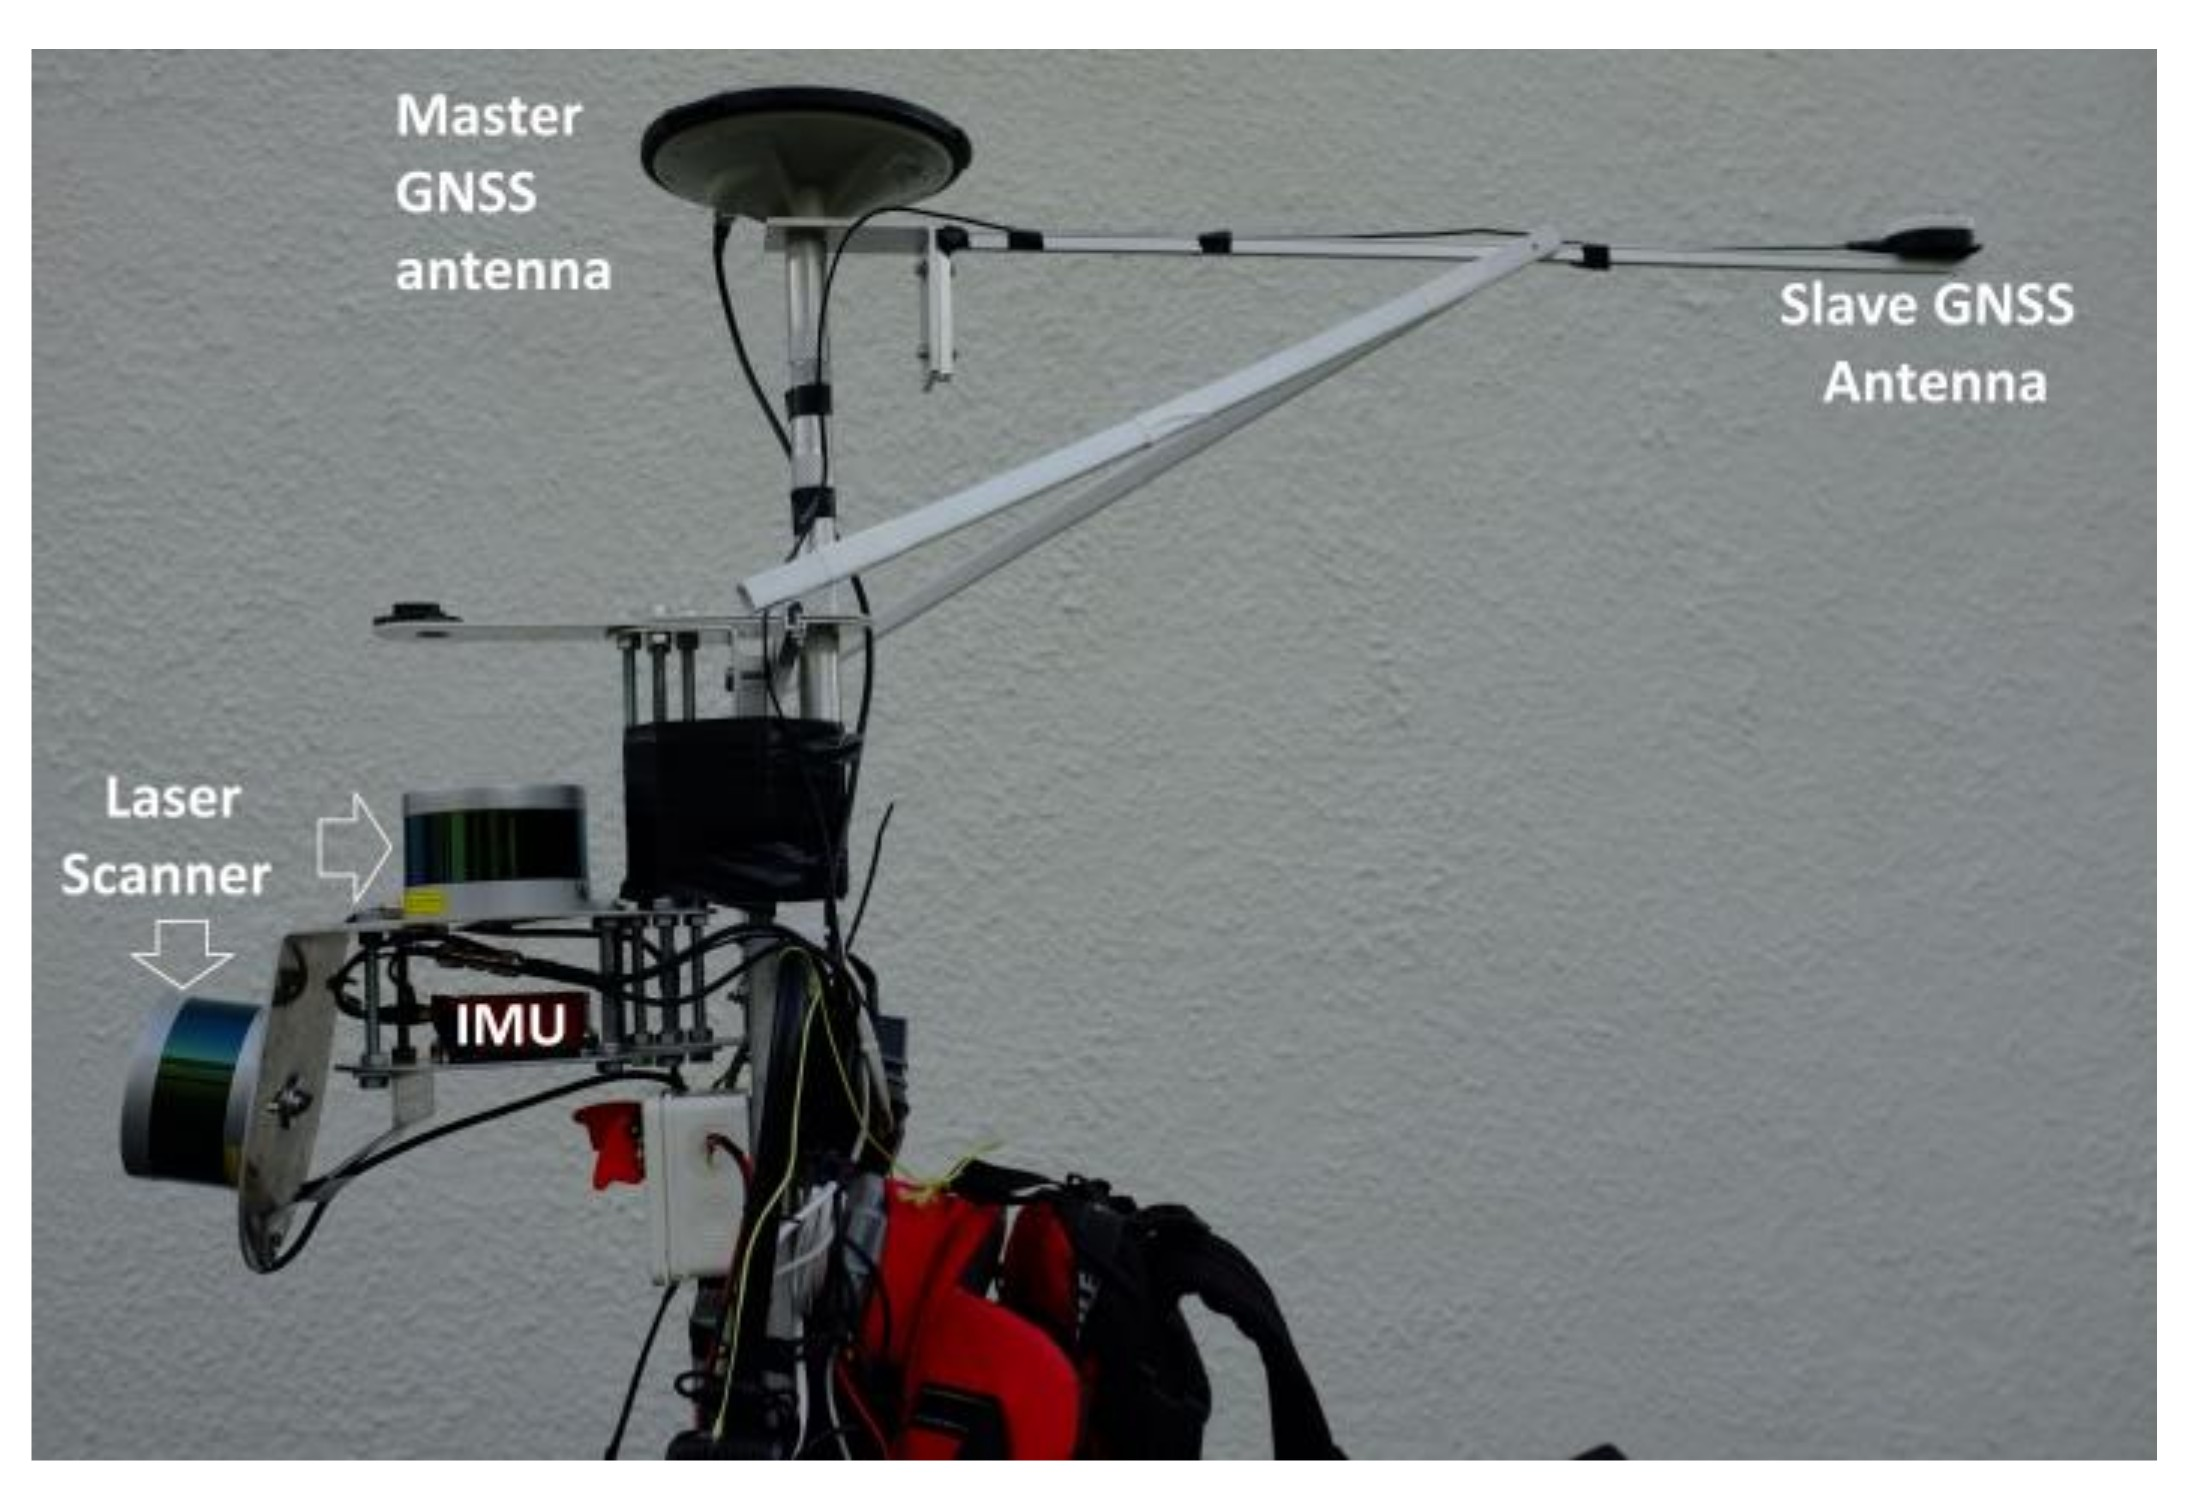
\includegraphics[width=\linewidth]{images/background/oveland_apparatus.jpg}
        \caption{Oveland's apparatus \cite{oveland_comparing_2018}}
        \label{fig: oveland apparatus}
    \end{subfigure}
    \begin{subfigure}{0.45\textwidth}
        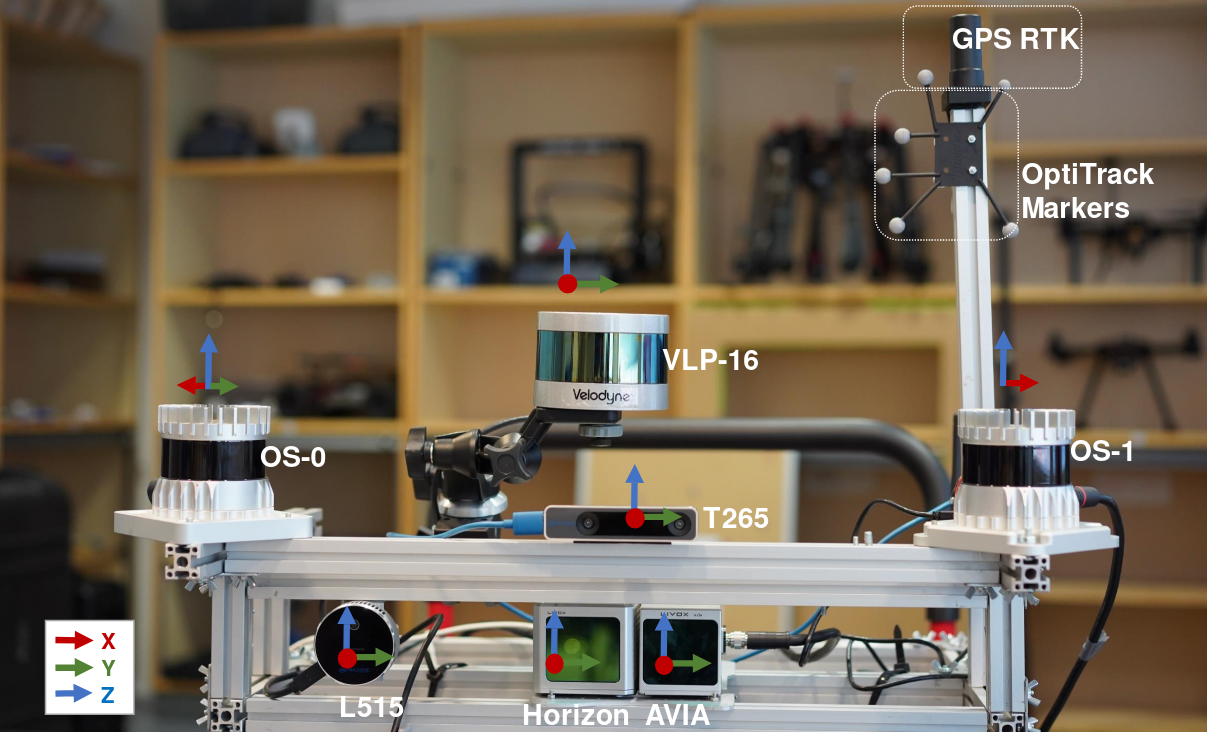
\includegraphics[width=\linewidth]{images/background/sier_apparatus.png}
        \caption{Sier's apparatus \cite{sier_benchmark_2022}}
        \label{fig: sier apparatus}
    \end{subfigure}
    \caption{Collection of the apparatus discussed in this section}
    \label{fig: all apparatus}
\end{figure}